%!TEX root = ../thesis_main.tex
%!TEX encoding = UTF-8 Unicode
\vspace{-0.2cm}
\begin{flushright}
\emph{``The more data we have, the more likely we are to drown in it.''}\\
Nassim Nicholas Taleb, in \textit{Fooled by Randomness: The Hidden Role of Chance in Life and in the Markets}, 2008
\end{flushright}
\vspace{0.4cm}

Assessing the robustness of a roadmap driving the transition pathway of a whole-energy system is complex, especially due to the curse of dimensionality. This curse comes from the number of variables of the system (\eg the installed capacity of technologies), the multiple-year approach specific to the pathway optimisation (\ie versus the snapshot approach) or the number of uncertain parameters. On top of this, the sector coupling interconnecting the installed capacities and the used resources among the different (non-)energy sectors can make harder the understanding of big trends of such a system. To navigate through this load of uncertain and interconnected data, it is necessary to assess the robustness of pathway roadmaps.

To deal with such uncertainties, decision-makers have several options: (i) resistance; (ii) resilience; (iii) static robustness; and (iv) adaptive robustness \cite{walker2012deep}. Where resistance consists in planning for the worst-case scenario, resilience aims at a fast recovery whatever the conditions in the future. Finally, in static robustness, one seeks for a roadmap that would perform ``satisfactorily'' in a wide range of plausible futures, whereas, a roadmap would be dynamically robust if it is prepared to adapt in case of a change in conditions. Where the adaptability of the policy was addressed in Chapter \ref{chap:chap_RL}, the objective of this chapter is to apply the method described in Section \ref{sec:meth:PCA} to deal with the static robustness of pathway roadmaps.  \citet{castrejon2020making} assessed policy mix folllowing the same philosophy of ``satisfactory level of performance'' as \cite{walker2012deep}. In their work, they mostly focused on the electricity sector, accounting for a variety of stakeholders and related interests using STET (Socio-Technical Energy Transition) models to capture more properly societal and behavioral aspects in relation with policy implementation, enriching purely techno-economy model, like EnergyScope, that usually assume rational choice within an overall cost minimization.  However, in the case of the transition pathway of a whole-eenrgy system, the challenges stand here in the definition of the ``performance metric'' as well as the ``satisfactory level of performance''. Between the sole total transition cost and the entire set of installed technologies that give too few and too much information, respectively, the performance metric here is defined through the \gls{PCA} approach. Then, when comes the ``satisfactory level of performance'', we propose a relative level of performance through a comparative analysis of different roadmaps. In other terms, one roadmap will not be robust or not in itself but rather more or less robust than another one. 

\section*{Contributions}
\label{sec:RobPol:contributions}
The main contributions of this chapter is the application of the methodology proposed in Section \ref{sec:meth:PCA} to the case study of the Belgian energy transition. First, we develop the different steps that lead to the principal components of the transition. We analyse these big trends of variation and highlight the fact that these variations stand for the entire pathway, a group of consecutive representative years or rather on a tipping-year. Then, and most importantly, we assess the robustness of different technological roadmaps by projecting their resulting myopic pathway against these directions of variation. The application of \gls{PCA} to provide a new metric for robustness applied to the case of Belgium is the added-value of this chapter.

\section{Definition of the principal components of the transition}
\label{sec:RobPol:PC_transition}
As detailed in Section \ref{subsec:meth:PCA:transition}, we have decided to define the directions of variation, \ie the robustness metrics, based on the installed capacities through the transition in the different end-use sectors, \ie electricity, \gls{HT} heat, \gls{LT} heat, passenger mobility, freight mobility, \gls{HVC}, ammonia and methanol. These capacities represent the technological roadmaps to supply these \gls{EUD} while respecting the \ce{CO2}-budget.  As introduced in Section \ref{subsec:meth:PCA:transition}, the data considered in this method come from the \gls{GSA} carried out on the perfect foresight optimisation of the Belgian transition pathway (see Chapter \ref{chap:atom_mol}). This gave 1260 different transitions resulting, for each of them, from the pathway optimisation subject to a sample of uncertain parameters (see Section \ref{subsec:uncert_charac}). Appendix \ref{app:UQ_tech_cap} gives the exhaustive distributions of the installed capacities among the different end-use sectors from the \gls{GSA}.

\subsection{Principal components of each representative year}
\label{subsec:RobPol:PC_year}
After the pre-preprocessing of the raw data (\ie data scaling and outliers management, see Section \ref{subsec:meth:PCA:transition}), the \gls{PCs} of each representative year of the transition, except 2020 as the initialisation year, can be computed. 

First of all, before investigating the \gls{PCs}, it is worth looking at the total variance of each representative year (see Table \ref{tab:design_variance}). Even though the absolute value of these variances has no physical meaning, we observe that the variations are more important at earlier stages of the transition. In other words, the further goes the transition, the more limited are the degrees of freedom to respect the \ce{CO2}-budget.

\begin{table}[htbp]
\caption{Whole-system design variance of the different representative years and their comparison with 2025.} 
\label{tab:design_variance}
\centering
\begin{tabular}{c c c}
\toprule
\textbf{Year}      & \textbf{Design variance} [$10^{-3}$]	 &	\textbf{vs. 2025}\\
\midrule
2025 	&	$10.4$	& - 	\\
2030 	&	$12.1$	& +15\%	\\
2035 	&	$9.7$	& -7\% 	\\
2040 	&	$6.1$	& -42\% 	\\
2045 	&	$5.1$	& -51\% 	\\
2050 	&	$4.8$	& -54\% 	\\
\bottomrule
\end{tabular}
\end{table}

Then, keeping the \gls{PCs} capturing at least 90\% of the total variance of each representative year, this gives between four, in 2035, and seven, in 2050, \gls{PCs} depending on the year (see Figure \ref{fig:PC_over_the_years}), and a total of 34 \gls{PCs}. At later stages of the transition, the increasing number of required \gls{PCs}, in line with their smaller share of explained variance, is another indication that the variance of the system design is more spread over a wider range of technologies and with a more limited amplitude. 

\begin{figure}[!htbp]
\centering
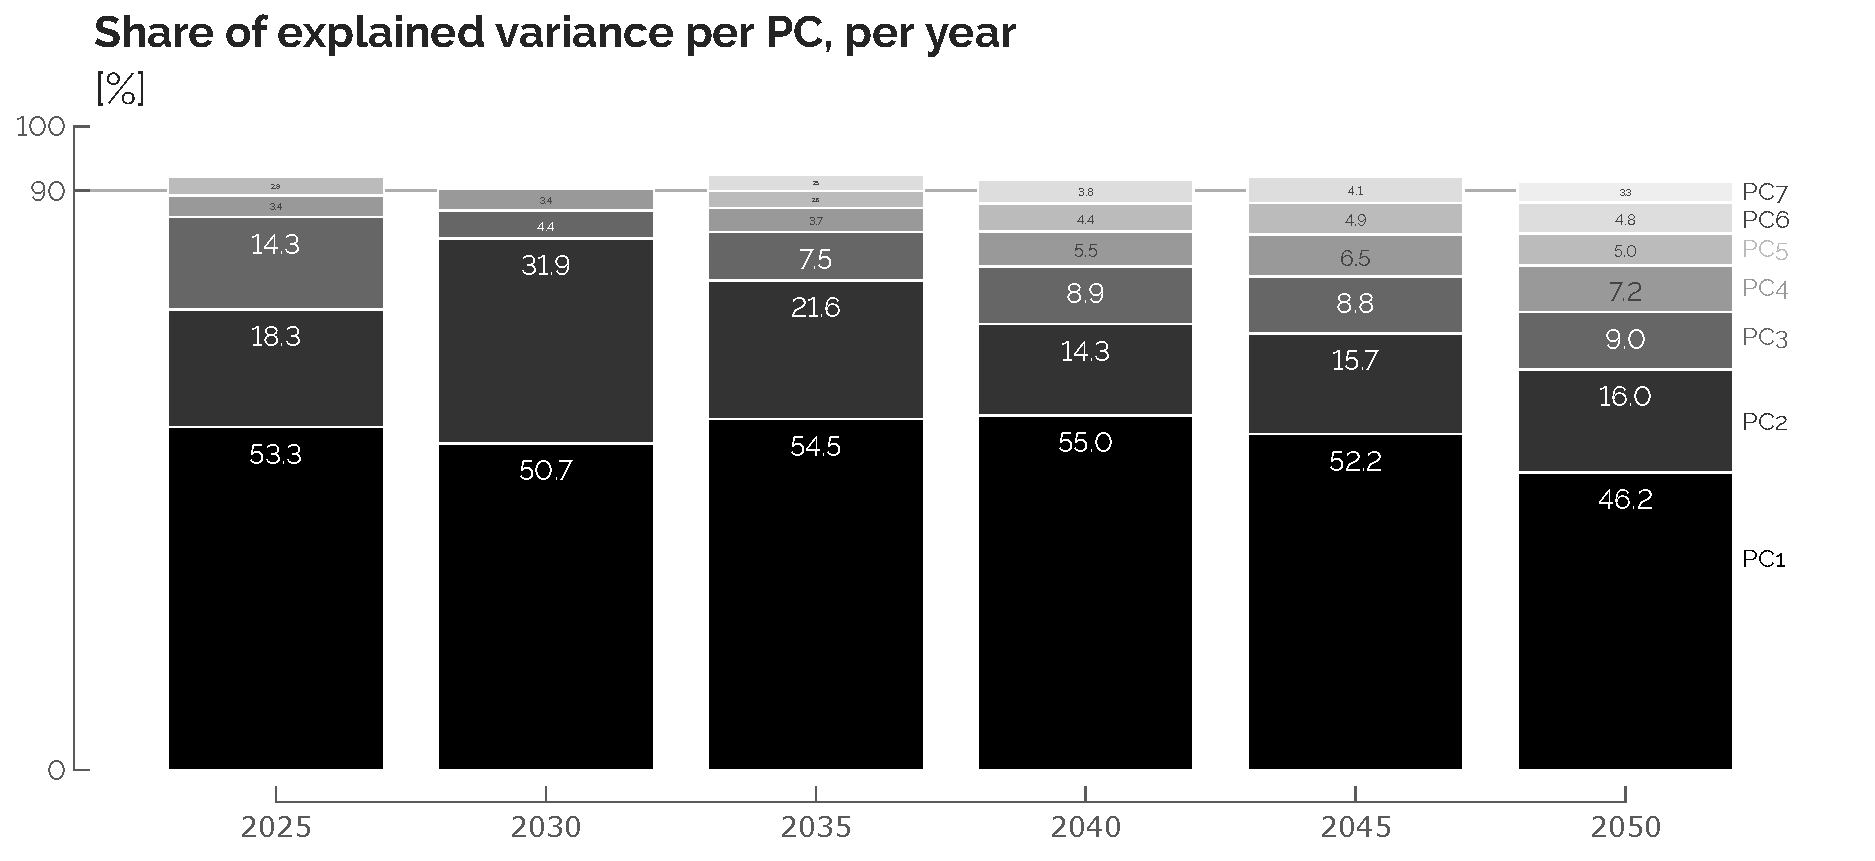
\includegraphics[width=\textwidth]{PC_over_the_years.pdf}
\caption{\gls{PCs} capturing at least 90\% of the total variance of their respective representative year of the transition. }
\label{fig:PC_over_the_years}
\end{figure}

Finally, we consider the respective contribution of the different technologies in the different $\text{PC}_{y}$, \ie their corresponding component in the different eigenvectors. Highlighting the top-5 technologies for $\text{PC}_{y,1}$, $\text{PC}_{y,2}$ and $\text{PC}_{y,3}$, we observe general trends over the whole transition as well as tipping year where there is a clear trade-off between several technologies (see Figure \ref{fig:Top5_PC_year}). As pointed out in Section \ref{subsec:meth:PCA:transition}, \gls{PCA} does not make any distinction between a vector of variation and its opposite. This is why $\text{PC}_{2025,1}$ and $\text{PC}_{2035,1}$ are actually very similar even though there are mostly on the opposite sides of the 0-axis.

\begin{figure}[!htbp]
\centering
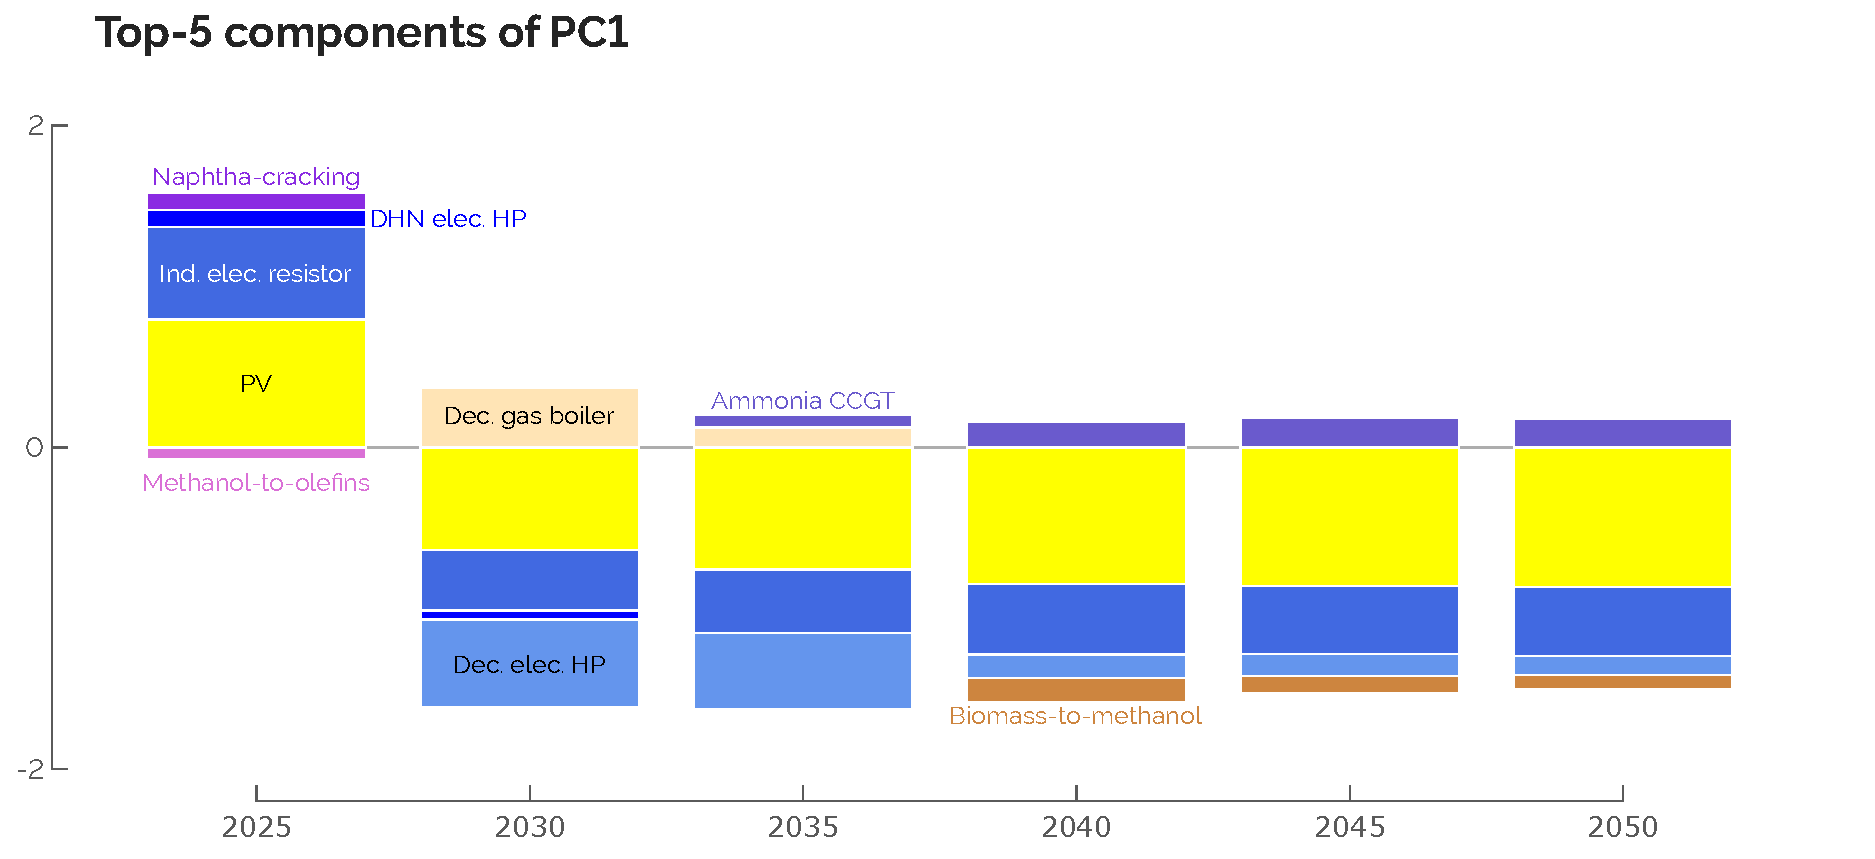
\includegraphics[width=0.8\textwidth]{Top5_PC1.pdf}
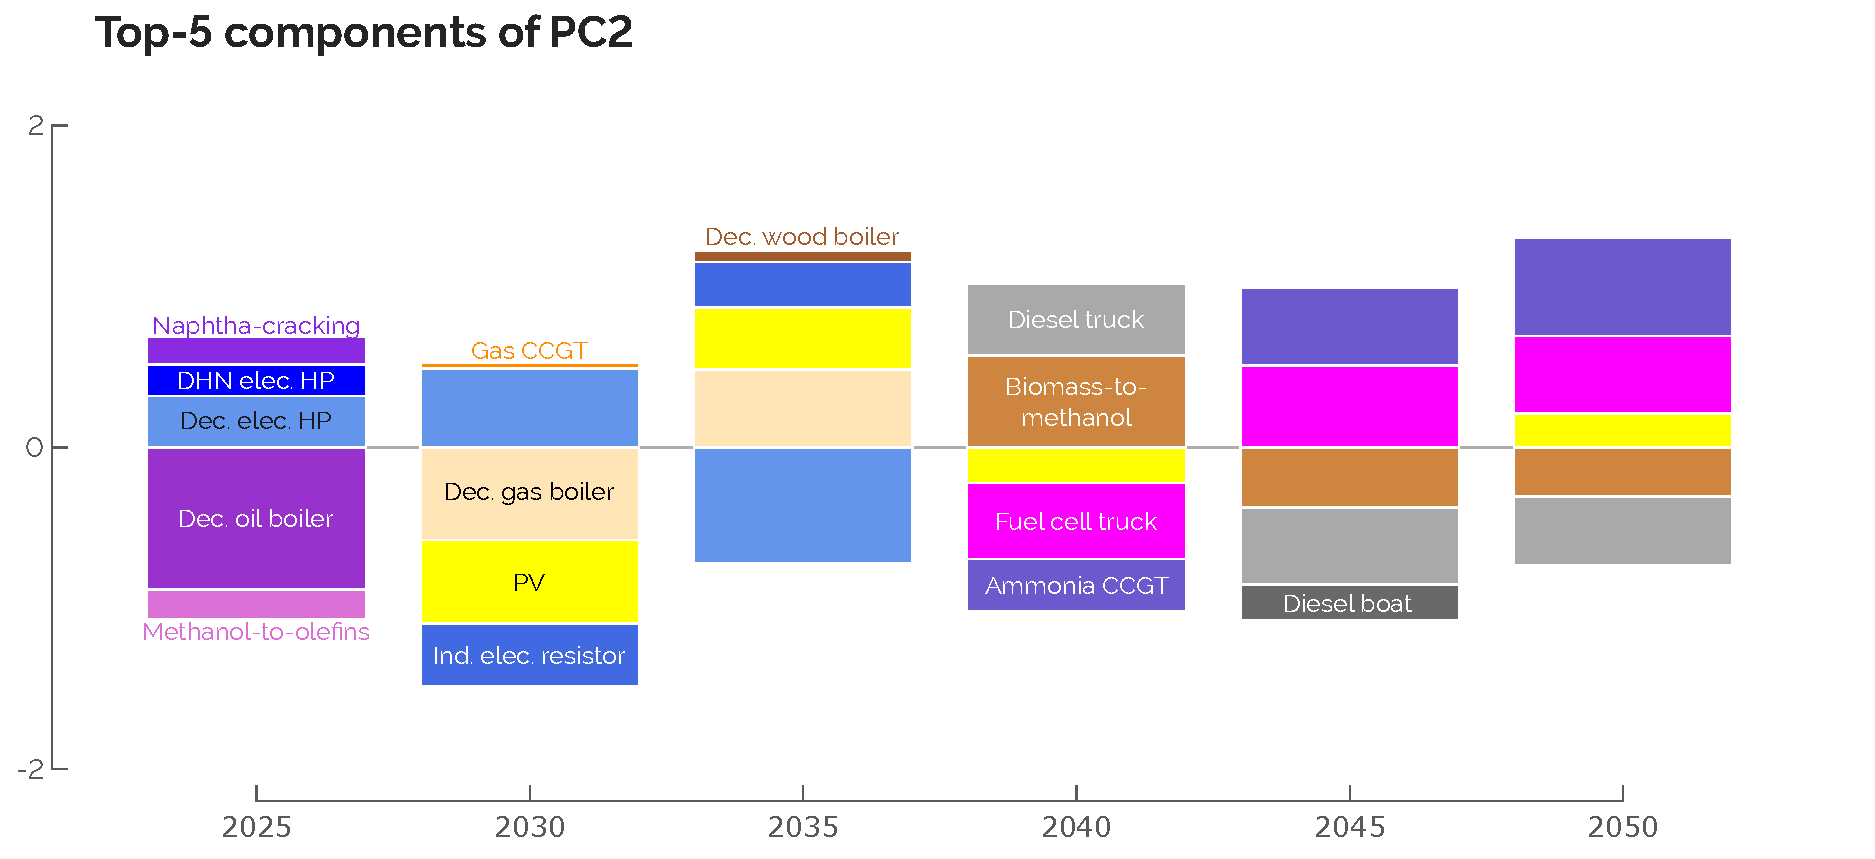
\includegraphics[width=0.8\textwidth]{Top5_PC2.pdf}
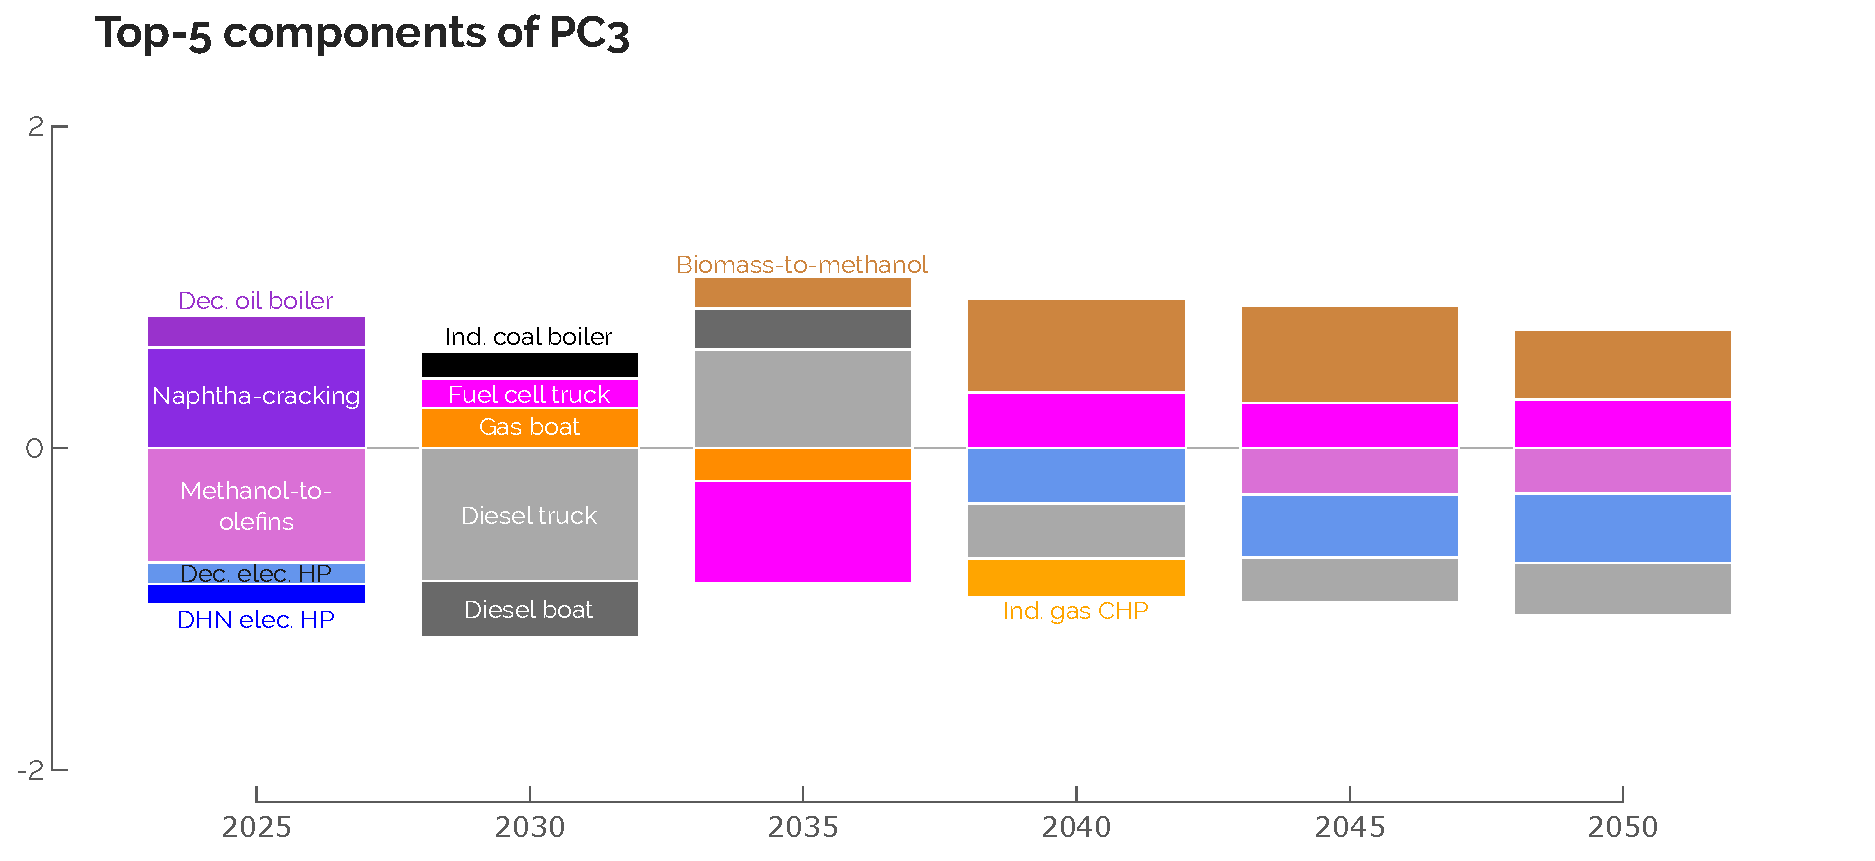
\includegraphics[width=0.8\textwidth]{Top5_PC3.pdf}
\caption{Contribution of the top-5 technologies to the first three \gls{PCs} over the different representative years. Where the variation of \gls{PV} panels supported by the electrification of the \gls{HT} heat via industrial electric resistors is the main varying drivers over the whole transition, there are tipping years like 2025 for the production of \gls{HVC} (\ie naphtha-cracker to \gls{MTO} or 2025-2030 for the production of \gls{LT} heat (\ie from oil and gas boilers to electric \gls{HP}.}
\label{fig:Top5_PC_year}
\end{figure}

Even though the following observations could be made by analysing the distribution of installed capacities (see Appendix \ref{app:UQ_tech_cap}) or the covariance matrices, the \gls{PCA} decomposition offers a more visual and summarising representation of the main trends of variation. Due to their intermittency, integrating more \gls{PV} panels leads to the installation of other technologies to benefit from free and renewable electricity when it exceeds the electrical \gls{EUD}. Therefore, we observe that the variation of installed \gls{PV} is directly linked with the variation of installed industrial electrical resistors and, to a smaller extent, of decentralised and \gls{DHN} electrical \gls{HP}. These variations cover the whole transition as the main varying factors given their significant contributions to the $\text{PC}_{1}$. Where this was an example for correlated technologies, we can also identify some key modal shifts where one technology is either substituted by others or in balance with another one. First, about the \gls{LT} heat sector, the early stages of the transition, \ie 2025-2030, sees the shift from mainly decentralised oil and gas boilers towards decentralised and \gls{DHN} electrical \gls{HP}. Later in the transition, there seems to be a tight competition between (bio)diesel and \gls{FC} trucks that drive the design variance to a smaller extent as they mostly appear in the second and third \gls{PCs} of the representative years. Not capturing a significant share of variance, there are other modal shifts (\eg \gls{BEV} substituting diesel and gasoline cars) that are not visible through the \gls{PCs}. Besides these modal shifts spread over several representative years, 2025 is the tipping year concerning the shift from naphtha-cracker and methanol-to-olefins to supply \gls{HVC}. Finally, there are also technologies contributing to \gls{PCs} because they are the main producing assets of their respective end-use sector and the demand varies significantly, \eg biomass-to-methanol.

\subsection{Principal components of the transition}
\label{subsec:RobPol:PC_transition}
Based on the \gls{PCs} of each representative year, $\text{PC}_{y}$, the \gls{PCs} of the transition, \ie the metrics to assess the robustness of roadmaps, can be computed. Before aggregating and averaging similar $\text{PC}_{y}$, it is necessary to rank them to ensure capturing most of the transition variance in the subsequent $\text{PC}_{\text{transition}}$.

Based on the design variance captured by each $\text{PC}_{y}$ in their respective representative year, we can rank them (see Table \ref{tab:ranking_PCs}). Summing all of these variances over the different years results in a ``pseudo'' total variance of the transition. To construct the \gls{PCs} of the transition, $\text{PC}_{\text{transition}}$, we keep the $\text{PC}_{y}$ that captures at least 80\% of this total variance of the transition (see Section \ref{subsec:meth:PCA:transition}).  This results in keeping 11 $\text{PC}_{y}$: the first PC of each representative year, the second of 2025, 2030, 2035 and 2040 and the third PC of 2025.

\begin{table}[htbp!]
\caption{Ranking of \gls{PCs} per design variance captured in their respective representative year and cumulative share of the captured total variance of the transition}
\label{tab:ranking_PCs}
\centering
\begin{tabular}{c c c c c}
\toprule
\multirow{2}{*}{\textbf{Ranking}} & \multirow{2}{*}{\textbf{Year}}  & \multirow{2}{*}{\textbf{PC}} & \multirow{2}{*}{\textbf{Design variance} [$10^{-4}$]} & \textbf{Cumulative share of} \\	
 &   &  &  & \textbf{total variance} [\%] \\	
 \midrule	
1 & 2030 & $\text{PC}_1$ & 61.1 & 13.9 \\
2 & 2025 & $\text{PC}_1$ & 55.7 & 26.5 \\
3 & 2035 & $\text{PC}_1$ & 52.7 & 38.4 \\
4 & 2030 & $\text{PC}_2$ & 38.4 & 47.2 \\
5 & 2040 & $\text{PC}_1$ & 33.4 & 54.7 \\
6 & 2045 & $\text{PC}_1$ & 26.5 & 60.7 \\
7 & 2050 & $\text{PC}_1$ & 22.2 & 65.8 \\
8 & 2035 & $\text{PC}_2$ & 20.9 & 70.5 \\
9 & 2025 & $\text{PC}_2$ & 19.1 & 74.8 \\
10 & 2025 & $\text{PC}_3$ & 15.0 & 78.2 \\
11 & 2040 & $\text{PC}_2$ & 8.7 & \textbf{80.2} \\
\midrule
$\vdots$ & $\vdots$ & $\vdots$ & $\vdots$ & $\vdots$\\
34 & 2050 & $\text{PC}_7$ & 1.6 & 100 \\
\bottomrule							

\end{tabular}
\end{table}

Given the similarity between $\text{PC}_y$, some $\text{PC}_{\text{transition}}$ result from the aggregation and averaging of the components of several $\text{PC}_y$.
